\documentclass[tikz,border=15pt]{standalone}
\usepackage{amsmath,amssymb}
\usetikzlibrary{calc}

\begin{document}
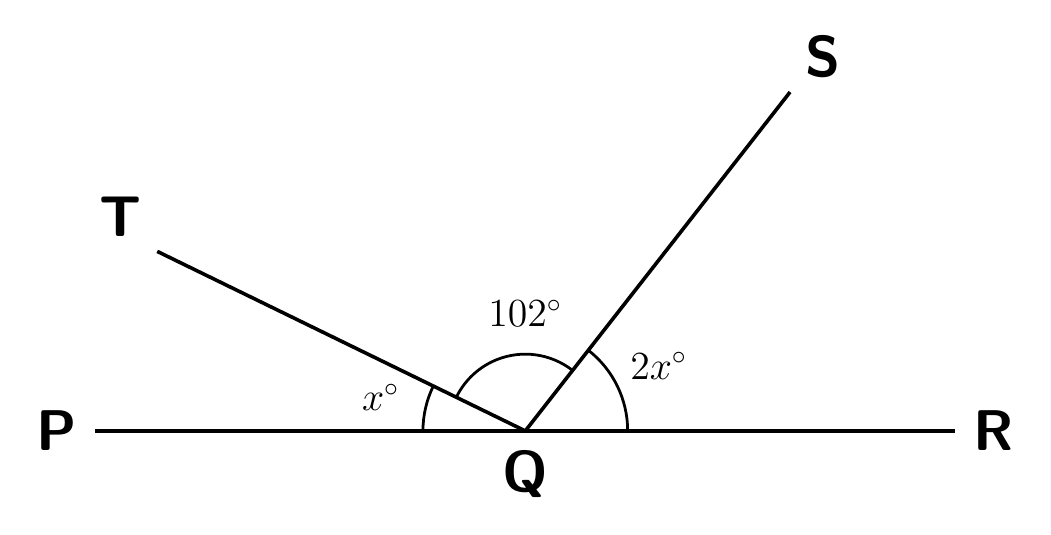
\begin{tikzpicture}[scale=1.3]
    % Straight line PQR
    \coordinate (Q) at (0, 0);
    \coordinate (P) at (-4.2, 0);
    \coordinate (R) at (4.2, 0);
    
    \draw[line width=1.4pt] (P) -- (R);
    
    % Rays QT and QS
    % x = 26 deg: angle of QS = 52 deg, angle of QT = 154 deg
    \def\lenT{4.0}
    \def\lenS{4.2}
    \coordinate (T) at ({154:\lenT});
    \coordinate (S) at ({52:\lenS});
    
    \draw[line width=1.3pt] (Q) -- (T);
    \draw[line width=1.3pt] (Q) -- (S);
    
    % Vertices labels
    \node[left=3pt, font=\huge\sffamily\bfseries] at (P) {P};
    \node[right=3pt, font=\huge\sffamily\bfseries] at (R) {R};
    \node[below=4pt, font=\huge\sffamily\bfseries] at (Q) {Q};
    \node[above left=2pt, font=\huge\sffamily\bfseries] at (T) {T};
    \node[above right=2pt, font=\huge\sffamily\bfseries] at (S) {S};
    
    % Angle arcs
    % Left angle x deg (154 to 180)
    \draw[line width=1.0pt] ($(Q) + (154:1.0)$) arc (154:180:1.0);
    \node[font=\Large\bfseries] at ($(Q) + (167:1.45)$) {$x^\circ$};
    
    % Middle angle 102 deg (52 to 154)
    \draw[line width=1.0pt] ($(Q) + (52:0.75)$) arc (52:154:0.75);
    \node[font=\Large\bfseries] at (0, 1.15) {$102^\circ$};
    
    % Right angle 2x deg (0 to 52)
    \draw[line width=1.0pt] ($(Q) + (0:1.0)$) arc (0:52:1.0);
    \node[font=\Large\bfseries] at ($(Q) + (26:1.45)$) {$2x^\circ$};
    
\end{tikzpicture}
\end{document}
